% Chapter Template

\chapter{Deep Semantics for Sentiment Analysis} % Main chapter title

\label{unl} % Change X to a consecutive number; for referencing this chapter elsewhere, use \ref{ChapterX}

\lhead{Chapter 6. \emph{Deep Semantics for Sentiment Analysis}} % Change X to a consecutive number; this is for the header on each page - perhaps a shortened title

%----------------------------------------------------------------------------------------
%	SECTION 1
%----------------------------------------------------------------------------------------

Existing methods for sentiment analysis  use supervised approaches which take into account all the subjective words and or phrases. Due to this, the fact that not 
all of these words and phrases actually contribute to the overall sentiment of the \textit{text} is ignored. We propose an unsupervised rule-based approach using 
deep semantic processing to identify only relevant subjective terms. We generate a UNL (Universal Networking Language) graph for the input \textit{text}. Rules are
applied on the graph to extract relevant terms. The sentiment expressed in these terms is used to figure out the overall sentiment of the \textit{text}. Results on
binary sentiment classification have shown promising results.

\section{Introduction}

Many works in sentiment analysis try to make use of shallow processing techniques. The common thing in all these works is that they merely try to identify sentiment-bearing
expressions as shown by \citep*{ruppenhofer2012semantic}. No effort has been made to identify which expression actually contributes to the overall sentiment of the text. 
In \citep*{mukherjee2012sentiment} these expressions are given weight-age according to their position w.r.t. the discourse elements in the \textit{text}. But it still takes into 
account each expression.
 
Semantic analysis is essential to understand the exact meaning conveyed in the \textit{text}. Some words tend to mislead the meaning of a given piece of \textit{text} as
shown in the previous example. WSD (Word Sense Disambiguation) is a technique which can been used to get the right sense of the word. \citep*{balamurali2011harnessing} have 
made use of WordNet synsets for a supervised sentiment classification task. \citep*{martin2010word} and \citep*{rentoumi2009sentiment} have also shown a performance improvement 
by using WSD as compared to word-based features for a supervised sentiment classification task. In \citep*{saif2012semantic}, semantic concepts have been used as additional 
features in addition to word-based features to show a performance improvement. Syntagmatic or structural properties of text are used in many NLP applications like machine 
translation, speech recognition, named entity recognition, etc. A clustering based approach which makes use of syntactic features of text has been shown to improve performance 
in \citep*{arhaves}. Another approach can be found in \citep*{mukherjee2012sentiment} which makes use of lightweight discourse for sentiment analysis. In general, approaches 
using semantic analysis are expensive than syntax-based approaches due to the shallow processing involved in the latter. As pointed out earlier, all these works incorporate all 
the sentiment-bearing expressions to evaluate the overall sentiment of the \textit{text}. The fact that not all expressions contribute to the overall sentiment is completely 
ignored due to this. Our approach tries to resolve this issue. To do this, we create a UNL graph for each piece of \textit{text} and include only the relevant expressions to 
predict the sentiment. Relevant expressions are those which satisfy the rules/conditions. After getting these expressions, we use a simple dictionary lookup along with attributes
of words in a UNL graph to calculate the sentiment.

In the next section, we will go through some of the related work in this direction.

\section{Related Work}

There has been a lot of work on using semantics in sentiment analysis. \citep*{saif2012semantic} have made use of semantic concepts as additional features in a word-based 
supervised sentiment classifier. Each entity is treated as a semantic concept e.g. \textit{iPhone, Apple, Microsoft, MacBook, iPad, etc.}. Using these concepts as features, 
they try to measure their correlation with positive and negative sentiments. In \citep*{verma2009incorporating}, effort has been made to construct document feature vectors 
that are sentiment-sensitive and use world knowledge. This has been achieved by incorporating sentiment-bearing words as features in document vectors. The use of WordNet synsets 
is found in \citep*{balamurali2011harnessing}, \citep*{rentoumi2009sentiment} and \citep*{martin2010word}. The one thing common with these approaches is that they make use of 
shallow semantics. An argument has been made in \citep*{choi2008learning} for determining the polarity of a sentiment-bearing expression that words or constituents within the
expression can interact with each other to yield a particular overall polarity. Structural inference motivated by compositional semantics has been used in this work. This work 
shows use of deep semantic information for the task of sentiment classification. A novel use of semantic frames is found in \citep*{ruppenhofer2012semantic}. As a step towards 
making use of deep semantics, they propose SentiFrameNet which is an extension to FrameNet. A semantic frame can be thought of as a conceptual structure describing an event,
relation, or object and the participants in it. It has been shown that potential and relevant sentiment bearing expressions can be easily pulled out from the sentence using 
the SentiFrameNet. All these works try to bridge the gap between rule-based and machine-learning based approaches but except the work in \citep*{ruppenhofer2012semantic},
all the other approaches consider all the sentiment-bearing expressions in the text.

\section{Use of Deep Semantics}\label{deep}
Before devising any solution to a problem, it is advisable to have a concise definition of the problem. Let us look at the formal definition of the sentiment analysis 
problem as given in \citep*{liu2010sentiment}. Before we do that, let us consider the following review for a movie, \textit{"1) I went to watch the new James Bond flick, 
Skyfall at IMAX which is the best theater in Mumbai with my brother a month ago. 2) I really liked the seating arrangement over there. 3) The screenplay was superb 
and kept me guessing till the end. 4) My brother doesn’t like the hospitality in the theater even now. 5) The movie is really good and the best bond flick ever."}
This is a snippet of the review for a movie named Skyfall . There are many entities and opinions expressed in it. 1) is an objective statement. 2) is subjective but 
is intended for the theater and not the movie. 3) is a positive statement about the screenplay which is an important aspect of the movie. 4) is a subjective
statement but is made by the author’s brother and also it is about the hospitality in the theater and not the movie or any of its aspects. 5) reflects a positive
view of the movie for the author. We can see from this example that not only the opinion but the opinion holder and the entity about which the opinion has been expressed 
are also very important for sentiment analysis. Also, as can be seen from 1),4) and 5) there is also a notion of time associated with every sentiment expressed.
Now, let us define the sentiment analysis problem formally as given in \citep*{liu2010sentiment}.
  
\textit{A direct opinion about the object is a quintuple \(<o_j,f_{jk},oo_{ijkl},h_i,t_l>\), where \(o_j\) is the the object, \(f_{jk}\) is the feature of the object
\(o_j\), \(oo_{ijkl}\) is the orientation or polarity of the opinion on feature \(f_{jk}\) of object \(o_j\), \(h_i\) is the opinion holder and \(t_i\) is the time 
when the opinion is expressed by \(h_i\).}
  
As can be seen from the formal definition of sentiment analysis and the motivating example, not all sentiment-bearing expressions contribute to the overall sentiment
of the \textit{text}. To solve this problem, we can make use of semantic roles in the \textit{text}. Semantic role is the underlying relationship that the underlying
participant has with the main verb. To identify the semantic roles, we make use of UNL in our approach.
  
\subsection*{UNL (Universal Networking Language)}

UNL is declarative formal language specifically designed to represent semantic data extracted from natural language texts. In UNL, the information is represented by 
a semantic network, also called UNL graph. UNL graph is made up of three discrete semantic entities, Universal Words, Universal Relations, and Universal Attributes. 
Universal Words are nodes in the semantic network, Universal Relations are arcs linking UWs, and Universal attributes are properties of UWs. To understand UNL better, 
let us consider an example. UNL graph for \textit{"I like that bad boy"} is as shown in the figure.
  
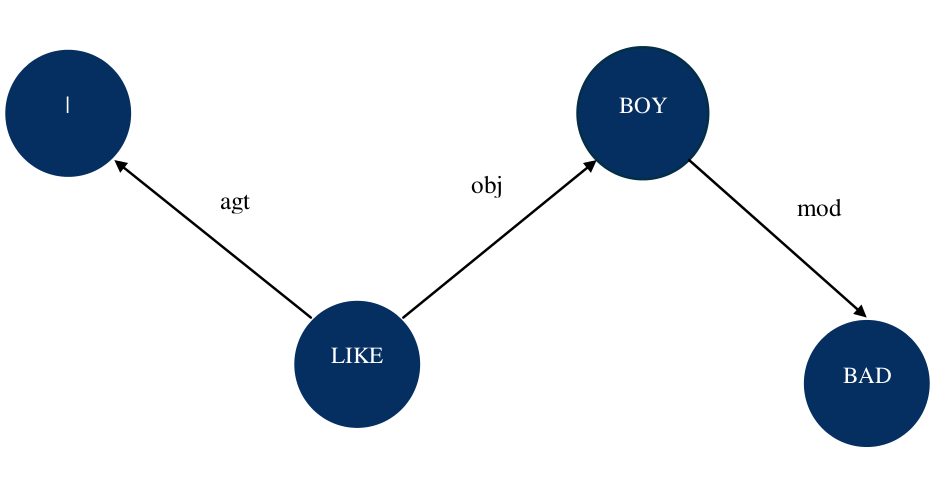
\includegraphics[width=\textwidth]{unlexample.png} 
\begin{center}
 Figure 6.1 UNL Example
\end{center}
  
Here, \textit{"I"}, \textit{"like"}, \textit{"bad"}, and \textit{"boy"} are the UWs. \textit{"agt"} (agent), \textit{"obj"} (patient), and \textit{"mod"} (modifier) are the
Universal Relations. Universal attributes are the properties associated with UWs which will be explained as and when necessary with the rules of our algorithm.
  
\subsubsection*{UNL relations}

Syntax of a UNL relation is as shown below,
    
\[\label{eqn:unlsyntax}
   <rel>:<scope><source>;<target>
\]
  
Where, \(<rel>\) is the name of the relation, \(<scope>\) is the scope of the relation, \(<source>\) is the UW that assigns the relation, and \(<target>\) is the UW that receives the relation \\
  
We have considered the following Universal relations in our approach,\\ 
1) \underline{\textit{agt} relation} \(:\) \textit{agt} stands for agent. An agent is a participant in action that provokes a change of state or location. The \textit{agt} 
relation for the sentence \textit{"John killed Mary"} is \textit{agt( killed , John )}. This means that the action of \textit{killing} was performed by \textit{John}.\\
2) \underline{\textit{obj} relation} \(:\) \textit{obj} stands for patient. A patient is a participant in action that undergoes a change of state or location. The \textit{obj} 
relation for the sentence \textit{"John killed Mary"} is \textit{obj( killed , Mary )}. This means that the patient/object of \textit{killing} is \textit{Mary}.\\
3) \underline{\textit{aoj} relation} \(:\) \textit{aoj} stands for object of an attribute. In the sentence \textit{"John is happy"}, the \textit{aoj} relation is 
\textit{aoj( happy , John )}.\\
4) \underline{\textit{mod} relation} \(:\) \textit{mod} stands for modifier of an object. In the sentence \textit{"a beautiful book"}, the \textit{mod} relation is 
\textit{mod( book , beautiful )}.\\
5) \underline{\textit{man} relation} \(:\) \textit{man} relation stands for manner. It is used to indicate how the action, experience or process of an event is carried out. 
In the sentence \textit{"The scenery is beautifully shot"}, the \textit{man} relation is \textit{man( beautifully , shot )}.\\
6) \underline{\textit{and} relation} \(:\) \textit{and} relation is used to state a conjunction between two entities. In the sentence \textit{"Happy and cheerful"}, 
the \textit{and} relation is \textit{and(Happy,cheerful)}.
    
\subsection*{Architecture}
  
As shown in the \textit{UNL} example, the modifier \textit{"bad"} is associated with the object of the main verb. It shouldn't affect the sentiment of the main agent. 
Therefore, we can ignore the modifier relation of the main object in such cases. After doing that, the sentiment of this sentence can be inferred to be positive.
The approach followed in the project is to first generate a UNL graph for the given input sentence. Then a set of rules is applied and used to infer the sentiment of the
sentence. The process is shown in Figure 6.2. The UNL generator shown in the Figure 6.2 has been developed at CFILT.\footnote{\url{http://www.cfilt.iitb.ac.in/}} Before, the given piece of text is passed on to the UNL 
generator, it goes through a number of pre-processing stages. Removal of redundant punctuations, special characters, emoticons, etc. are part of this process. This is
extremely important because the UNL generator is not able to handle special characters at the moment. We can see that, the performance of the overall system is limited
by this. A more robust version of the UNL generator will certainly allow the system to infer the sentiment more accurately.
  
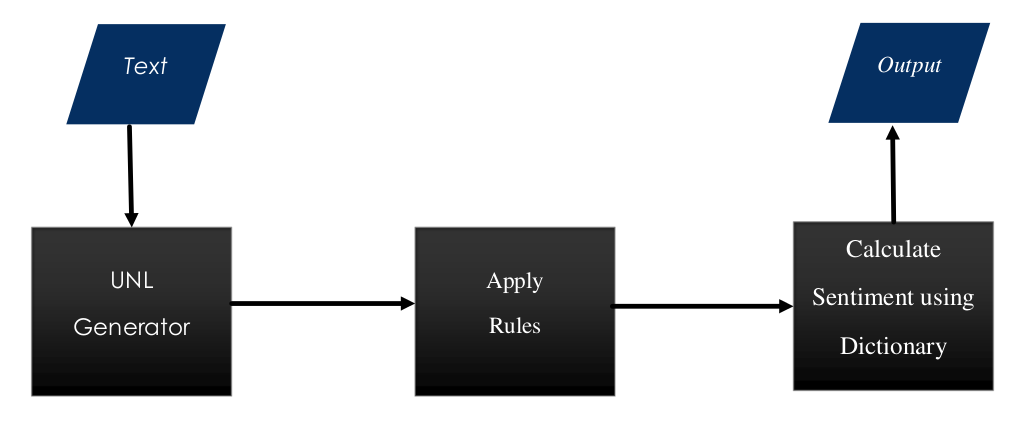
\includegraphics[width=\textwidth]{unlusage.png} 
\begin{center}
 Figure 6.2 Architecture
\end{center}
  
\subsection*{Rules}

There is a separate rule for each relation. For each UW (Universal word) considered, if it has a \textit{@not} attribute then its polarity is reversed. Rules used by the system
are as follows,\\
1) If a given UW is source of the \textit{agt} relation, then its polarity is added to the overall polarity of the text.
\underline{e.g.,} \textit{"I like her"}. Here, the agt relation will be \textit{agt ( like , I )}. The polarity of like being positive, the overall polarity of the text is positive.
\underline{e.g,} \textit{"I don't like her"}. Here the agt relation will be \textit{agt ( like@not , I )}. The polarity of like is positive but it has an attribute \textit{@not}
so its polarity is negative. The overall polarity of the text is negative in this case. \\
2) If a given UW is source or target of the \textit{obj} relation and has the attribute \textit{@entry} then its polarity is added to the overall polarity of the text. This rule 
merely takes into account the main verb of the sentence into account, and the it's is polarity considered.
\underline{e.g.,} \textit{"I like her"}, here the obj relation will be \textit{obj ( like@entry , her )}. The polarity of like being positive, the overall polarity of the text is positive \\
3) If a given UW is the source of the \textit{aoj} relation and has the attribute \textit{@entry} then its polarity is added to the overall polarity of the text.
\underline{e.g.,} \textit{"Going downtown tonight it will be amazing on the waterfront with the snow"}. Here, the \textit{aoj} relation is \textit{aoj ( amazing@entry , it )}. 
\textit{amazing} has a positive polarity and therefore overall polarity is positive in this case.\\
4) If a given UW is the target of the \textit{mod} relation and the source UW has the attribute \textit{@entry} or has the attribute \textit{@indef} then polarity of the 
target UW is added to the overall polarity of the text.
\underline{e.g.,} \textit{"I like that bad boy"}. Here, the aoj relation is \textit{mod ( boy , bad )}. \textit{bad} has a negative polarity but the source UW, boy does not have an 
\textit{@entry} attribute. So, in this case negative polarity of bad is not considered as should be the case.
\underline{e.g.,} \textit{"She has a gorgeous face"}. Here, the mod relation is \textit{mod ( face@indef , gorgeous )}. \textit{gorgeous} has a positive polarity and face has an 
attribute \textit{@indef}. So, polarity of gorgeous should be considered. \\
5) If a given UW is the target of the \textit{man} relation and the source UW has the attribute \textit{@entry} then polarity of the target UW is added to the overall polarity of 
the text. Or if the target UW has the attribute \textit{@entry} then also we can consider polarity of the target UW. 
\underline{e.g.,} \textit{"He always runs fast"}. Here, the \textit{aoj} relation is \textit{mod ( run@entry , fast )}. \textit{fast} has a positive polarity and the source UW, run 
has the \textit{@entry} attribute. So, in this case positive polarity of fast is added to the overall polarity of the sentence.
Polarities of both the source and target UW of the \textit{and} relation are considered. \\
6) In \textit{"Happy and Cheerful"}, the \textit{and} relation is \textit{and(Happy, Cheerful)}. \textit{Happy} and \textit{Cheerful}, both have a positive
polarity, which gives this sentence an overall positive polarity.
 
The polarity value of each individual word is looked up in a dictionary of positive of negative words used is \citep*{liu2010sentiment} After all the rules are applied, summation of all the calculated polarity values is done. 
If this sum is greater than 0 then it is considered as positive, and negative otherwise. This system is negative biased due to the fact that people often tend to express negative sentiment 
indirectly or by comparison with something good.

\section*{SUMMARY}

In the beginning, we expressed the motivation behind this approach. After that, related work was discussed. Then we explained the approach to use deep semantics in detail.
The experiments performed using this approach will be explained in the next chapter.